\newpage
\section{Collaborative filtering}
\paragraph{}The need of having recommender systems lies between the need of obtaining recommendations from trustworthy sources and the availability of a large amount of user data.
\paragraph{}Like on any demand and supply system, on the one hand, lies the demand of accurate and trustworthy recommendations. On the other hand are the tons of user data that can serve this demand.
\paragraph{}Over the years have been developed techniques that can utilize those data, in order to provide good recommendations. Those techniques are highly dependent on the volume of data they use. 

\paragraph{}The more the data the more accurate the recommendation. But its system's training phase is largely impacted by the volume mentioned before. Thus, any algorithm or system is will provide good recommendations as long as it is trained with the right dataset.

\paragraph{} Those algorithms were initially based only on statistical models that were available at the time. Whereas the data were growing rapidly, and the sample started to approach the population.
\subsection{Content based}

\paragraph{}The most common and easy to interpret the way of recommendation is collaborative filtering. In this area of algorithms, you are trying to utilize data from other users in order to come to a recommendation. Those data might be attributes that characterize the item of interest. 
\paragraph{}In the case of users, those attributes may be their age or occupation, whereas for a product might be its color, prize or weight in kilograms. In order to put this to a mathematical expression, we could write the following.

\begin{equation}
w=R^{-1}M^{T}
\end{equation}

\paragraph{}Raw data though are not always clear of normalized. Due to this fact, we would consider to normalizing the approach we used above. If we were about to add a normalization factor to that expression we will end up with the one below.

\begin{equation}
w=(\lambda I + R^{T}R)^{-1} R^{T}M 
\end{equation}

\paragraph{}That kind of algorithms is easier to interpret. They also can handle well a cold-start problem. But they are computational heavy, meaning that the scaling of them is limited.

\subsection{Latent Factors}

\paragraph{}Another approach to recommender algorithms is the latent factors group. This group of algorithms does not take into consideration the meta-data we have for any user or item. 
\paragraph{}In that area, we are trying to determine relationships between a user and an item based only on the rating. Those relationships may not be the age or the color.

\begin{figure}[h]
	\centering
	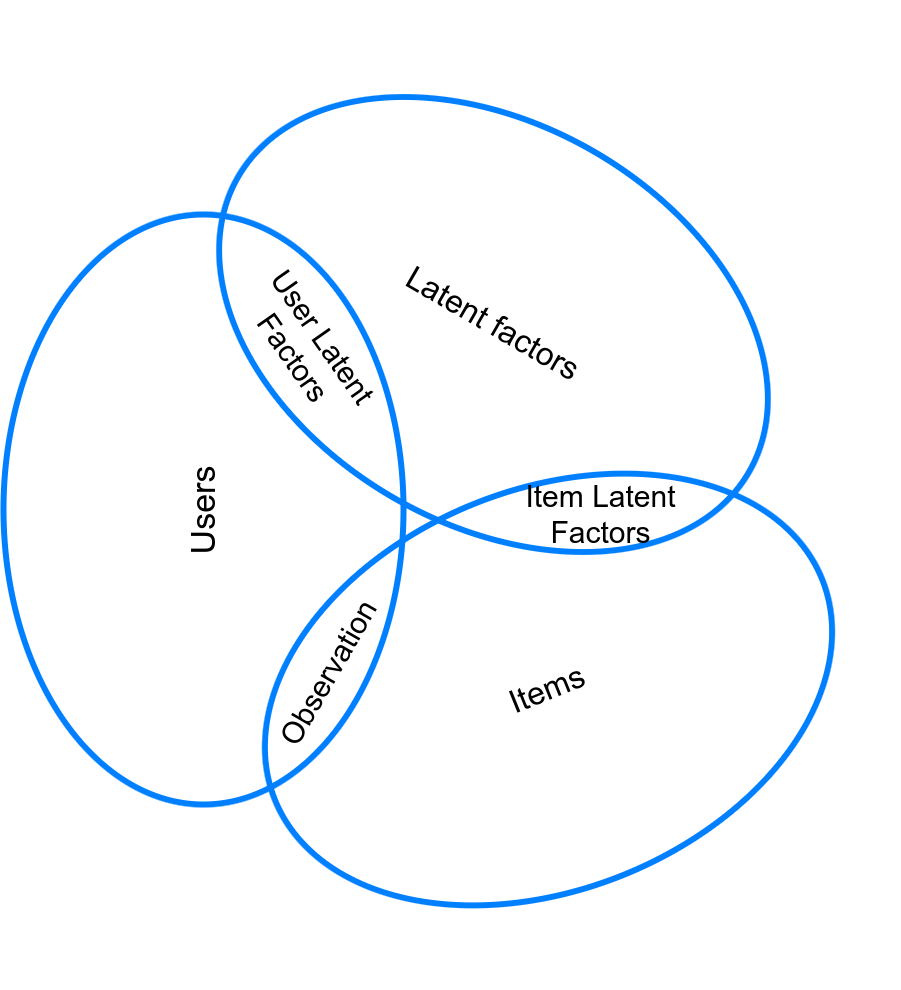
\includegraphics[width=0.5\textwidth]{images/LatentFactors.png}
	\caption{\bfseries LatentFactors}
	\label{LatentFactors}
\end{figure}


\paragraph{} Alternating least squares (ALS) algorithm belongs to the group above. In this case, we assign initially random values of rating between user and items. Then it takes the error between the actual value and the one assigned to it. 
\pagebreak
\paragraph{}Then the algorithm runs again using as input the errors and tries to minimize them. Below we can see a how this algorithm is defined.

\begin{algorithm}
	\caption{ALS for Matrix Completion}\label{ALS}
	\begin{algorithmic}[1]
		\State Initialize X,Y
		\Repeat
		\For{\texttt{u=1...n}}
		\State $x_{u} = (\sum_{r_{ui}}y_{i}y_{i}^{T} + \lambda I_k)^{-1} \sum_{r_{ui}}r_{ui}y_{i} ,\in r_{u*}$
		\EndFor
		\For{\texttt{i=1...m}}
		\State $y_{i} = (\sum_{r_{ui}}x_{u}x_{u}^{T} + \lambda I_k)^{-1} \sum_{r_{ui}}r_{ui}x_{u} ,\in r_{*i}$
		\EndFor
		\Until {convergence}
	\end{algorithmic}
\end{algorithm}

\paragraph{}As we can see above, this algorithm has a $\lambda$ parameter used for normalization during the process. We can see the difference below where we have both the expression with and without normalization factor.

\paragraph{} ALS is a very efficient recommender algorithm. Due to its nature, it can be easily parallelized reducing the execution time needed \cite{DistributedAlgorithmsAndOptimization:4}. It also requires no meta-data about any user or item. Although, ALS suffers from the cold start problem.

\begin{equation}
	\min_{X,Y} \sum_{r_{ui}observed}(r_{ui}-x_{u}^{T}y_{i})^{2}
\end{equation}

\begin{equation}
	\min_{X,Y} \sum_{r_{ui}observed}(r_{ui}-x_{u}^{T}y_{i})^{2} + \lambda(\sum_{u}||x_{u}||^2 + \sum_{i}||y_{i}||^2)
\end{equation}

\paragraph{} Moving forward this thesis, we are going to discuss how those two algorithms were implemented and validate the results they gave.